\clearpage

\section{MC Samples and event weighting}
% \label{sec:mcsample}
%-------------------------------------------------------------------------------
% *refraseMT*
The samples used are divided into two main groups: Standard Model (SM) background and beyond SM signal. The SM background includes the QCD multijet samples, produced with a falling $\pt$ spectrum. The beyond SM signals are $W'\to WZ\to q\bar{q}'q\bar{q}$, $Z'\to t\bar{t}$ (top quarks considered in the full hadronic channel ($t\to W(\to q\bar{q}')b$)) and RS-Graviton $\to hh \to b\bar{b}b\bar{b}$, i.e. final states have only jets in all the samples. The details of the samples are given in Table \ref{tab:mcsamples}; the masses considered span from 0.5 to 5 TeV to improve and diversify the kinematic space covered.

% A set of kinematic distributions for the $W'$ is shown in Figure \ref{fig:wprimekinematic}: on the left the $\pt$ distribution where the kinks correspond to the Jacobian peak of the mass considered and the $\eta$ distribution on the right. The green dots represent the distribution before the selection, which is $\pt >$ 250 GeV and $|\eta|<$ 2.0 and the red dots after this selection. This selection typical for many searches for BSM physics.  All the other samples and the background can be found in the Appendix. 
% In what follows, it will also be used the nomenclature \textit{boosted W/Z} for the $W'$ sample, \textit{boosted tops} for the $Z'$ sample, \textit{boosted Higgs} for the $G_{RS}$ sample and \textit{massive $W$} for the $W' \to \tilde{W}\tilde{W}$ with $m_{\tilde{W}}=m_t$.
% *refraseMT*

\begin{table}
\centering
\hspace*{-3em}\begin{tabular}{l|lllr}  
% \toprule
\hline
\hline
Process & ME Generator & ME PDFs &  UE Tune & Resonance Masses\\
  & \& Fragmentation &  & & \\

\hline
QCD multijet &Pythia 8&NNPDF23LO & A14& N/A \\
\hline
$W'\to WZ$ &Pythia 8&NNPDF23LO & A14& 1.5, 2.5, 3, 4, 5 TeV \\
\cline{1-1}
$Z'\to t\bar{t}$ &Pythia 8&NNPDF23LO & A14& 1.5, 1.75, 2.5, 3, 4, 5 TeV \\
\cline{1-1}
$G_{RS} \to hh(\to b\bar{b})$ &Pythia 8&NNPDF23LO & A14& 0.5, 1, 1.5, 2, 2.5, 3 TeV\\
\cline{1-1}
$W' \to \tilde{W}\tilde{W}$ &Pythia 8&NNPDF23LO & A14& 1.5, 2.5, 3, 4, 5 TeV \\
with $m_{\tilde{W}}=m_t$ & & & & \\
\hline
\hline
% \bottomrule
\end{tabular}
\caption[Overview of the Monte Carlo Samples used]{Overview of the Monte Carlo Samples used. The first line shows QCD standard model process, the second, the third and the forth the beyond SM samples considered; the last line the ``massive $W/Z$'' sample.}
\label{tab:mcsamples}
% \end{center}
\end{table}
The substructure observables are compared via their performance in QCD rejection. While the $p_{\mathrm{T}}$ distribution of the multi-jet sample falls exponentially, the $p_{\mathrm{T}}$ of the signal samples features characteristic peaks related to the resonance masses. To avoid bias in the comparison, the signal sample is given weights such that the truth $p_{\mathrm{T}}$ distribution of the leading jet matches the one of the background sample (see Figure \ref{fig:p_T} in the Appendix). Furthermore, the spectrum is split into six different $p_{\mathrm{T}}$ regions to study the behavior with rising energy.
\clearpage
% \newpage
%-------------------------------------------------------------------------------
\clearpage
\section{Object Definition}
\label{sec:objdef}
%-------------------------------------------------------------------------------

This section gives an overview of the objects used for the observables based on subjet-assisted tracks, which are the large-radius jet mass, the Energy Correlation Functions and the n-Subjettiness, as they are used within ATLAS.
% , the next section will give the details of the modified approach of the subjet-assisted techniques.

\subsection{Standard Large-Radius jet}

% Large-radius jet, or arge-$R$ jets are jets constructed with a radius parameter of the reclustering algorithm much bigger than the standard 0.4; within ATLAS the size of large-$R$ jets is 1.0 for anti-k$_t$ and 1.2 for C/A (the area of C/A is $\sim$20\% smaller than anti-k$_t$).

% It is worth noting that, for a standard anti-k$_t$ 0.4 jet the active area \cite{antiktalgo} is $A_{anti-k_t}=\pi R^2 \simeq 0.5$, while it is $\simeq 3.14$ for 1.0 jet, i.e. around six times bigger.

% Already from this ``geometrical'' point of view, the necessity of further techniques can be understood: the effect of soft radiation contamination from Pile-Up (PU) and Underlying Event (UE) will be in this case six times bigger and spoil the efficiency of the jet mass measurements.

Large-radius jet, or large-$R$ jets are jets constructed with a radius parameter of the reclustering algorithm of 1.0 for those built using the anti-k$_t$ algorithm and 1.2 for the C/A algorithm \cite{antiktalgo}.
Since the active area of this jets is typically six times bigger than their counterparts of radius 0.4 which is the usual choice of jet radii within ATLAS, the necessity of further techniques is required to have control over the effect of soft radiation contamination from Pile-Up (PU) and Underlying Event (UE).

\subsubsection{Grooming and Selection}

% This section is based on the 7 TeV article on jet Substructure \cite{substructure1}.
\paragraph{Grooming}
In order to use large-$R$ jets, it is necessary to gain additional information on the interior of these objects, i.e. using techniques that exploit their substructure allowing a jet-by-jet discrimination of the energy deposit most likely coming from the hard-scattering to other soft radiation.

A common feature in substructure is the use of \textit{subjet}, i.e. jets obtained from a parent jet (e.g. the large-$R$ jet), using its constituent but running the jet reclustering algorithm with a smaller radius parameter; in one large-$R$ jet, typically there are two or more subjets depending on the originating process and its $\pt$.

Techniques have been developed, both using subjets or directly constituents of a jet, which are referred to as \textit{grooming} algorithms.

Grooming algorithms are designed to retain the characteristic substructure within such a large-$R$
jet while reducing the impact of the fluctuations of the parton shower and the UE, thereby
improving the mass resolution and mitigating the influence of pile-up.

The grooming algorithms presented here are the most important ones in ATLAS: the \textit{Trimming}; other used as well, the \textit{Split-Filtering} and the \textit{Pruning} can be found in \cite{substructure1}. Details on Trimming, the most used within ATLAS and in this note, are given in the Appendix.

\paragraph{Selection}

The selection applied is typical for many Beyond the Standard Model searches: $p_T>$ 250 GeV and $|\eta|<$ 2.0 for the large-radius jet.
No other requirements were made for the purpose of the performance studies here shown if not stated differently, e.g. the mass cut selection.
% The green dots represent the distribution before the selection, which is $\pt >$ 250 GeV and $|\eta|<$ 2.0 and the red dots after this selection. This selection typical for many searches for BSM physics.  All the other samples and the background can be found in the Appendix. 
% In what follows, it will also be used the nomenclature \textit{boosted W/Z} for the $W'$ sample, \textit{boosted tops} for the $Z'$ sample, \textit{boosted Higgs} for the $G_{RS}$ sample and \textit{massive $W$} for the $W' \to \tilde{W}\tilde{W}$ with $m_{\tilde{W}}=m_t$.


\subsubsection{Calorimeter Mass}

% Once the collection of constituents from the large-$R$ jet is groomed, i.e. the most likely sources of soft radiation from PU and UE are eliminated, one can start working with those and start worrying about how to get physical-related properties from it, e.g. the mass.
Once the collection of topo-clusters from the large-$R$ jet is groomed, i.e. cleaned from PU contamination through the trimming technique, it is possible to use them for the measure of physical related properties such as the jet mass, since the possible sources of soft radiation from PU and UE have been reduced.


The \textit{calorimeter mass} or $m^{calo}$ is a widely used variable which takes as input the topo-cluster information. Given that each topo-cluster $i$ has a 3D information on the energy deposit, $E_i$, $\eta$ and $\phi$, the mass can be simply calculated from 4-vector properties:
$$m^{calo}=\sqrt{\left(\sum_{i\in J}E_i\right)^2-\left(\sum_{i\in J}p_{T,i}\right)^2} $$
where $J$ labels the Large-$R$ jet and the topo-clusters are assumed massless.

\subsubsection{Track Mass}
\label{sec:tracks}
% This section briefly presents the tracks and how they are related to the properties of the large-$R$ jets.
% This section briefly presents the tracks and their relation with the large-$R$ jet's properties.
% There are significant advantages of tracks and why they are interesting and possible candidate for precise mass reconstruction and a big disadvantage.
There are significant advantages and few disadvantages of the use of tracks for large-radius jet mass reconstruction, inherited both from the detector experimental properties and from the underlying physical processes. 
Main advantages are: performance of angular separation and the association of the tracks to the primary vertex for rejection of soft radiation background.
Tracks can additionally required to be well reconstructed from the detector and they are classified in  \textrm{LOOSE},  \textrm{MEDIUM} and \textrm{TIGHT} for increasing quality criteria.
The mass $m^{track}$ is then calculated summing up the 4-momenta of those tracks which passed the selection and are ghost associated to the groomed jet.

% First of all the performance of angular separation at low $\pt$ is intrinsically better for tracks than the calorimeter one; moreover tracks can be associated to the primary vertex excluding Pile Up and soft radiation background.


% The second main advantage is that tracks can be associated with the primary vertex, thus simply excluding those from PU or other beam-induced soft radiation background (this is not the case for the UE).

% The requirement made on tracks to achieve optimal performance are grouped into two categories, the quality of the track, i.e. if it was fully reconstructed from the detector and separated from others with no ambiguities, and the association conditions with the primary vertex; further details are given in the appendix.

% Given the set of tracks which pass this selection, the mass $m^{track}$ is calculated summing up the 4-momenta of those tracks which are ghost associated to the groomed jet.

% The main, big disadvantage is that the tracker system is completely blind to the neutral component of the jet, which, as said, amounts to c.a. a third of the total. As seen in Figure \ref{fig:trackandcalo}, the track mass (red distribution) is not only shifted towards lower values than the calorimeter mass (green distribution), but its width also degrades. 
The important disadvantage comes from the complete blindness of the tracker system to the 
% Apart from this benefits which derive from the tracker system, there is also an important disadvantage which comes from the underlying physics:
 electrically neutral component (mostly $\pi^0$) of the jet. As seen in Figure \ref{fig:trackandcalo}, the track mass (red distribution) is not only shifted towards lower values than the calorimeter mass (green distribution), but its width also degrades. 

Tracks could be used either for independent mass reconstruction or, most importantly, as an additional information to the calorimeter measurement.

\begin{figure}[!ht]
  \centering
      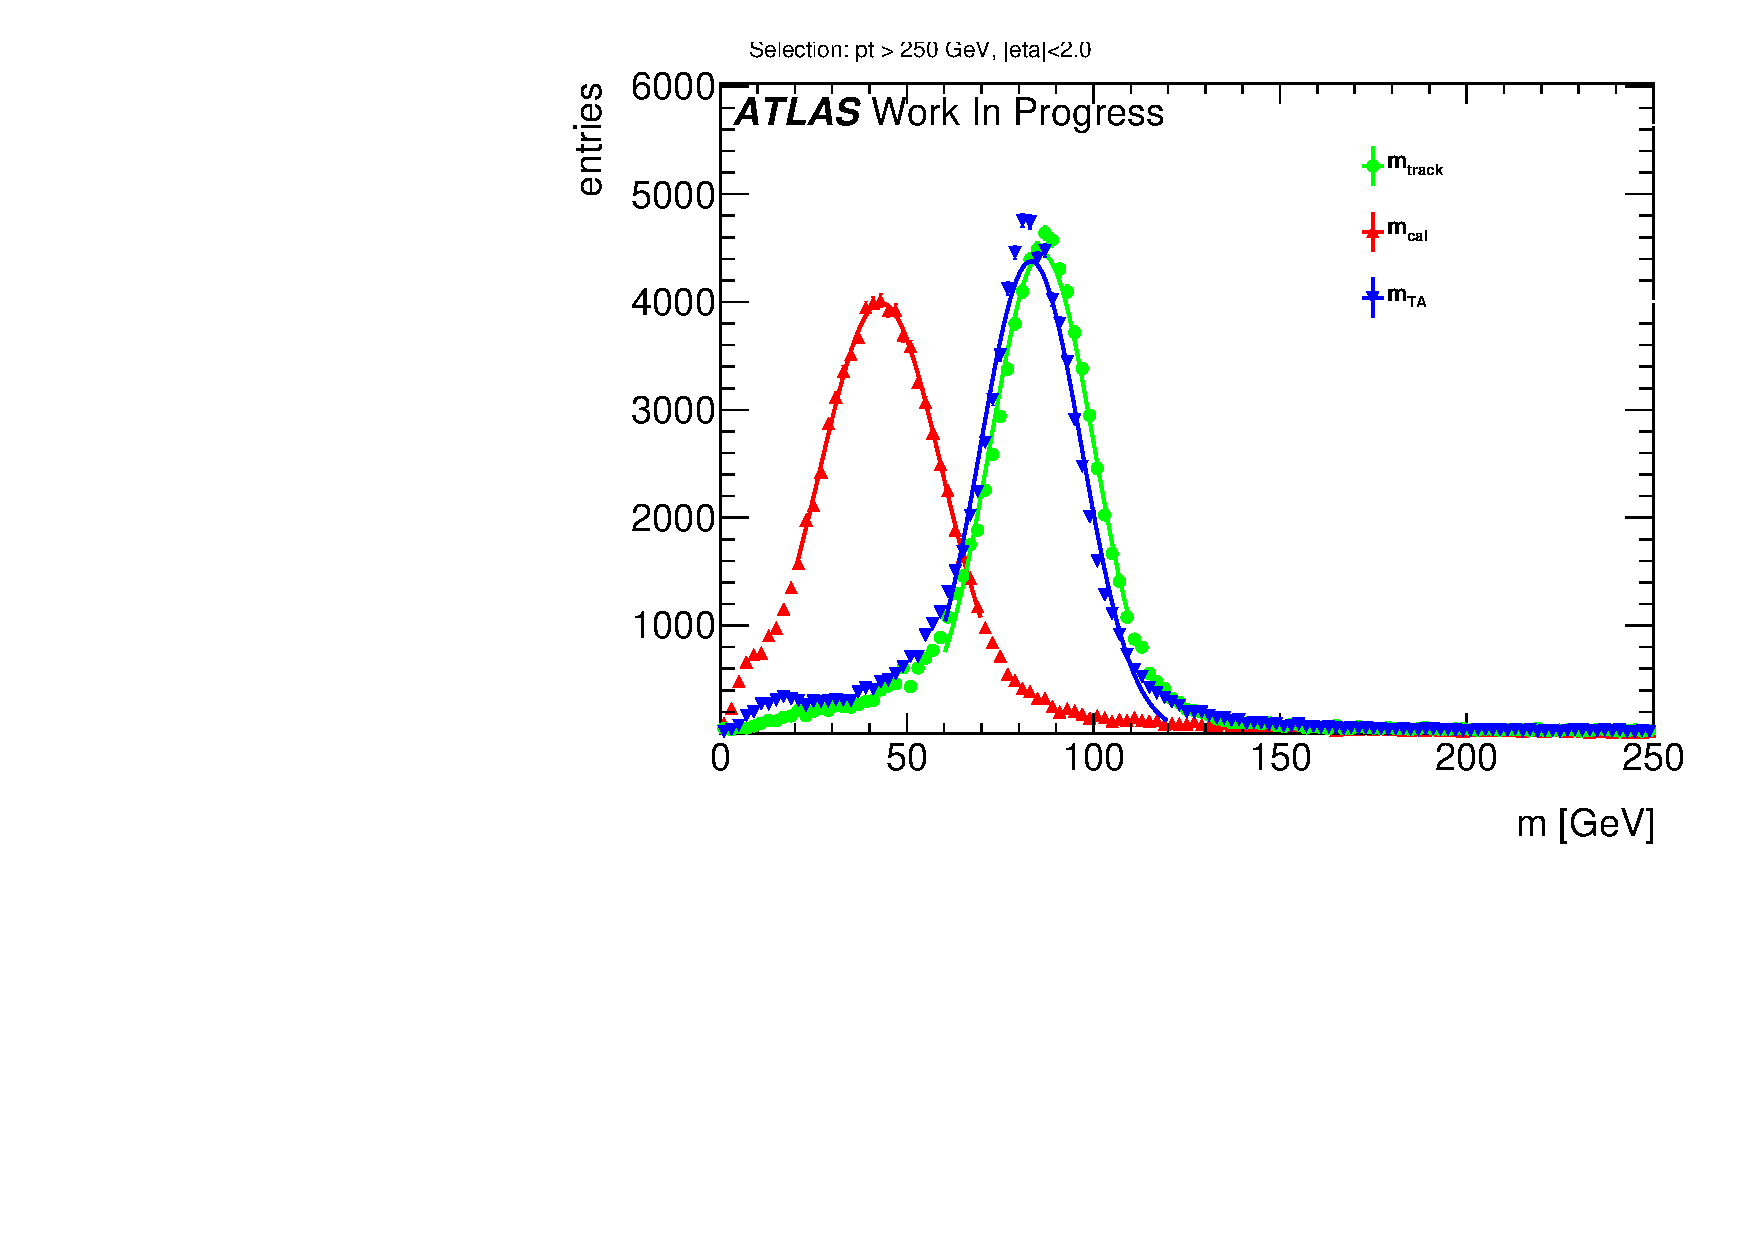
\includegraphics[width=0.7\textwidth]{jet_part/1cfrt_h_TrackJets_m.pdf}
  \caption[Mass distribution for $W/Z$ decays]{Mass distribution for $W/Z$ decays: in green the $m^{calo}$ in red the $m^{track}$ and in blue the $\mta$. }
  \label{fig:trackandcalo}
\end{figure}


\subsubsection{Track-Assisted Mass ($\mta$)}
The track-assisted mass, $\mta$, was one of the first attempts to combine the information form the tracker system and from the calorimeter. It is defined as $\mta=\frac{p_T^{calo}}{p_T^{track}}\times m^{track}$, where the $p_T^{track}$ and the $m^{track}$ are calculated from the tracks which are associated to the large-radius jet, adding up their 4-momenta (hence exploiting the superior angular resolution of the tracker system); the $p_T^{calo}$ is the transverse momentum as measured from the calorimeter system. The ratio $p_T^{calo}/p_T^{track}$ restores the fraction of the missing neutral component in the $m^{track}$.
The $\mta$ has a better performance on the reconstruction of boosted objects such as $W/Z$ in the extreme kinematic regime ($\sim $ 1 TeV) and above in the transverse momentum of the decaying electroweak object. Another advantage of this observable shows up as it comes to the systematic uncertainties: in particular jet mass scale and jet mass resolution uncertainty on $\mta$ can be estimated by propagating the track reconstruction uncertainties and calorimeter-jet $\pt$ uncertainties through the definition of the variable given above. The tracking uncertainties are smaller for $\mta$ rather than $\mcal$ because a larger extent of the uncertainty cancels in the ratio $m^{track}/p_T^{track}$.
Apart all of these advantages, the track-assisted mass shows its limits when it comes to intermediate transverse momentum regimes and below ($\pt < 1 $ TeV) in $W/Z$ and for Higgs and top quarks throughout the whole kinematic space.
% The track-assisted mass, $\mta$, was one of the first attempts to combine the information form the tracker system and from the calorimeter. 
% The track mass is missing the neutral component, i.e. each measurement is missing the fraction $\frac{neutral+charged}{charged}$, but it has very good angular resolution but $\pt$ resolution degrades linearly with the transverse momentum. The calorimeter mass, on the other hand, has the limitation of the angular resolution of the topo-clusters but relative energy resolution increases at higher energies. The missing neutral fraction from the tracker system could be corrected on a jet-by-jet basis taking advantage of the two detector sub-system optimalities: this leads to the definition of the \textit{track-assisted mass} ($m^{TA}$):
% \begin{equation}
 % m^{TA}=\frac{p_T^{calo}}{p_T^{track}}\times m^{track}
% \end{equation}
% The better resolution of the $\mta$ takes place at the scale of above $\sim1$ TeV of transverse momentum for $W/Z$, while the performance is suboptimal to the calorimeter mass for all the other samples considered.
% Another advantage with respect to 
Full description of this variable is given in the ATLAS CONF Note \cite{art35}.
% The main limitation of the calorimeter mass comes from the angular resolution of the topo-clusters, which, for extreme kinematic regimes, start approaching each other at the point that they hit the granularity of the detector. The main advantage is that on the contrary the relative energy resolution increases at higher energies.

% The tracks instead have a very good angular resolution, but $\pt$ relative resolution degrades linearly with the transverse momentum. 

% One could then think about creating a variable which exploits the advantages of both and minimizes the disadvantages. As seen, the track mass is missing the neutral component, i.e. each measurement is missing the fraction $\frac{neutral+charged}{charged}$, but it could be corrected on a jet-by-jet basis: this leads to the definition of the \textit{track-assisted mass} ($m^{TA}$):
% \begin{equation}
%  m^{TA}=\frac{p_T^{calo}}{p_T^{track}}\times m^{track}
% \end{equation}

% It can be intuitively understood as follows: the term $m^{track}$ has the superior angular resolution, but misses the neutral component; the ratio $p_T^{calo}/p_T^{track}$, representing exactly the $(neutral+charged)/charged$ ratio, ``restores'' the correct value of the mass back to $charged+neutral$.
% \begin{figure}[!ht]
%   \centering
%       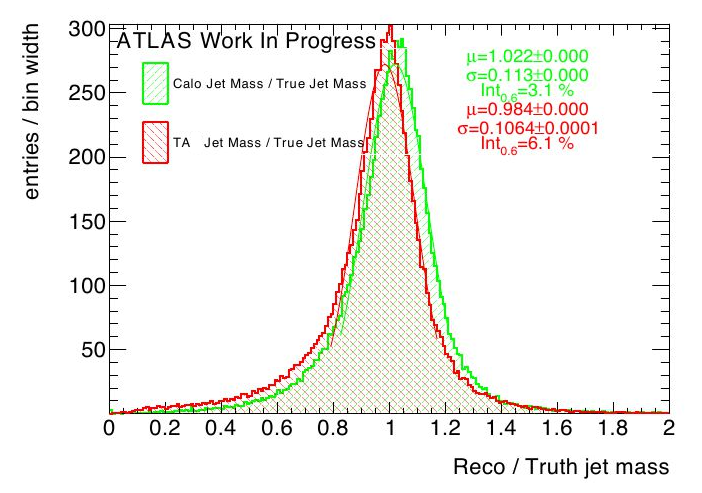
\includegraphics[width=0.7\textwidth]{jet_part/mta/allbinptmta.png}
%   \caption[$\mcal$ and $\mta$ mass responses]{Track-assisted mass response plot for boosted $W/Z$: in green the calorimeter mass, in red the track-assisted mass. On the right are shown properties of the fit to the Gaussian core; it can be seen than the width of the $\mta$ distribution is smaller, and the mean is slightly below the calorimeter mass.}
%   \label{fig:mta1}
% \end{figure}

% From Figure \ref{fig:mta1} the comparison of the track-assisted mass and the calorimeter mass; the width of the distribution is smaller, making this observable a good candidate for usage.


% \subsection{Advantages and Limitation of $\mta$}
% The $\mta$ has a good handle on boosted $W/Z$, looking at all the transverse momentum spectrum for these results.

% \begin{figure}[!ht]
%   \centering
%       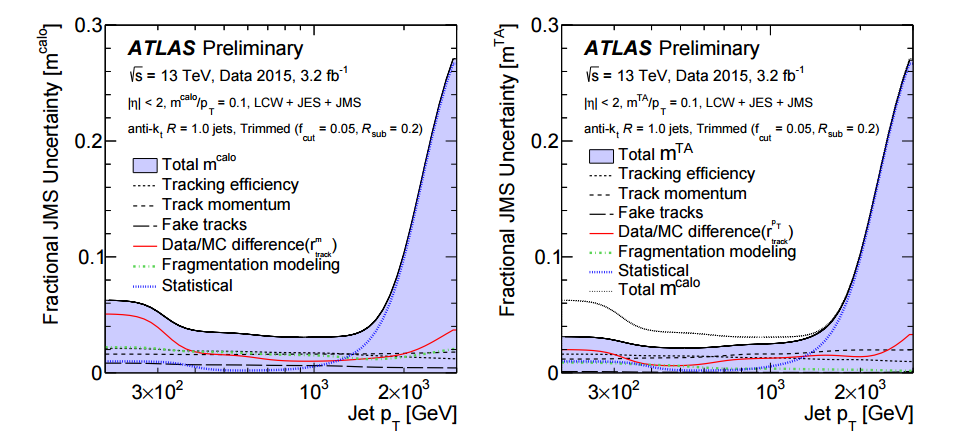
\includegraphics[width=0.9\textwidth]{jet_part/uncert.png}
%   \caption[Comparison of the uncertainties for $\mcal$ and $\mta$]{Comparison of the uncertainties for $\mcal$, on the left, and $\mta$, on the right the rise on the high jet $\pt$ is due to statistics. From the \cite{art35}.}
%   \label{fig:uncert}
% \end{figure}

% Another big advantage which supports the use of the track-assisted mass is the relatively small uncertainties: in Figure \ref{fig:uncert} the comparison of $\mcal$ (left) and $\mta$ (right) fractional uncertainties on the JMS, shows how the tracking uncertainties are much smaller because of the ratio $m^{track}/p_T^{track}$. On the right plot the black line indicates the JMS fractional uncertainty for the $\mcal$, and is always above the $\mta$. Of course this introduces another argument in the development of new techniques, which is to look for a good balance between performance and small uncertainties: a perfect observable in terms of behavior which has very big uncertainties is not really useful.


% When looking in the extreme kinematic regime, at very high $\pt$, as in the top plot in Figure \ref{fig:mta2}, the $\mta$ shows its real strength, achieving much smaller value of the IQnR.
% However, there are some severe limitations which are worth noting, especially looking at the performance in different regions of transverse momentum: this is shown in the bottom plot of Figure \ref{fig:mta2}, where at a low $\pt$ it exhibits a much worse behavior.

% \subsubsection{Performance in $W \to q'\bar{q}$ Decays}

% \begin{figure}
%     \centering
%     \begin{subfigure}[b]{0.5\textwidth}
% 	\centering
%         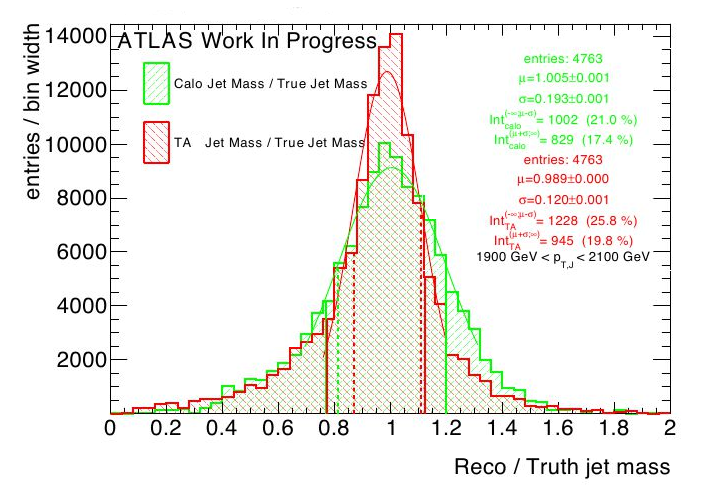
\includegraphics[width=\textwidth]{jet_part/mta/highptmta.png}
   
% %         \label{fig:tiger}
%     \end{subfigure}
%     \begin{subfigure}[b]{0.5\textwidth}
% 	\centering
%         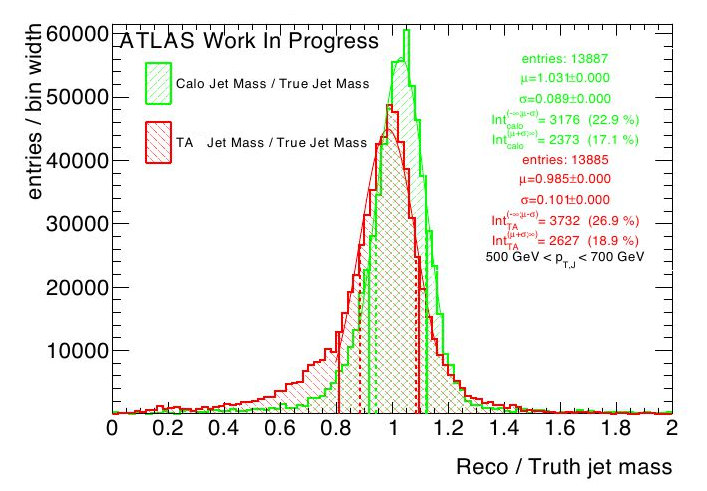
\includegraphics[width=\textwidth]{jet_part/mta/lowptmta.png}
 
% %         \label{fig:gull}
%     \end{subfigure}
%     \caption[Mass response plots for the $\mta$]{Mass response plots for selected ranges of $\pt$: on the bottom, a ``low'' range, 500 GeV $<\pt<$ 700 GeV, on the top an high $\pt$, 1900 GeV $<\pt<$ 2100 GeV. A difference in performance can be clearly seen.} 
%     \label{fig:mta2}
% \end{figure}


% The performance in all the bins of $\pt$ can be studied looking at Figure \ref{fig:mta3}; these plots have as horizontal axis the transverse momentum and as vertical one the value of the $\iqr$ calculated from the correspondingly response. For $W/Z$ jets, there is a crossing point around $\pt\sim$1 TeV, which can be understood as the point in which the two subjet present start merging (subjet multiplicity shown in Figure \ref{fig:multi} in Appendix).



% \subsubsection{Performance in $t\to q'\bar{q}b$ Decays}

% For top quarks the situation is much different: with respect to $W/Z$ jets, in fact, there are two main disparities: on one side, the mass of the top quark is much higher than the one of the electroweak bosons, hence making the separation $\Delta R=\frac{2m}{\pt}$ bigger; on the other side, the decay is not anymore two-prong (two-subjet-like) but rather a three-prong  (three-subjet-like) decay, one from the b-jet and the other two from the $W$ decay.
% $\mta$ is here never performing better than $\mcal$, as can be seen e.g. in Figure \ref{fig:mta3}, right.


% \begin{figure}[!ht]
%   \centering
%       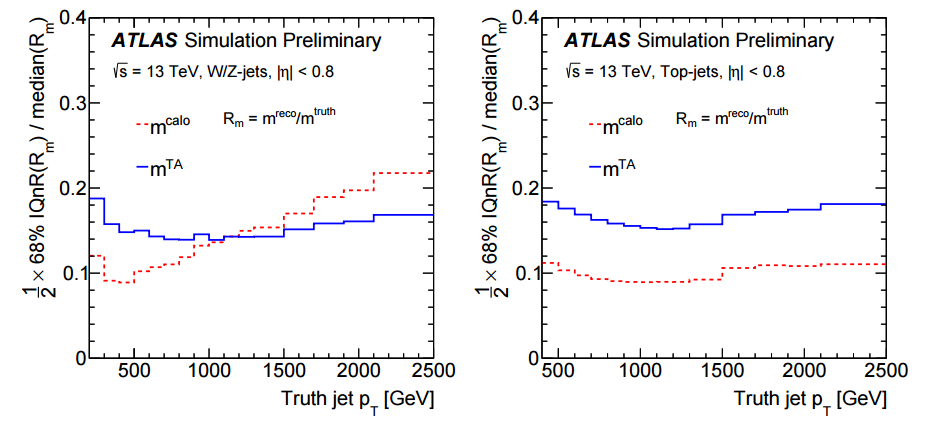
\includegraphics[width=\textwidth]{jet_part/mtawandtop.png}
%   \caption[$m^{calo}$ and $m^{TA}$ comparison for $W/Z$ jets and top jets]{The comparison between the performance of $m^{calo}$ and $m^{TA}$ for $W/Z$ jets (left) and top jets (right); on the x-axis the transverse momentum and on the y-axes the $\iqr$ of the mass distribution, from \cite{art35}. A better observable has lower values on the y-axis. }
%   \label{fig:mta3}
% \end{figure}

% \subsubsection{Performance in $h\to b\bar{b}$ Decays}

% For boosted Higgs the $\mcal$ outperforms the $\mta$ in the spectrum of transverse momentum. Although the decay is two-pronged, the mass of the Higgs is higher than the electroweak bosons, moreover another difference lays in light quarks initiated jets and heavy quarks initiated ones, like the b-quarks from Higgs decay.
% % the b-jet poses an additional complication which comes from the branching ratio of B mesons to muons, which leave very little energy in the calorimeter system but additional tracks.

% \begin{figure}[!ht]
%   \centering
%       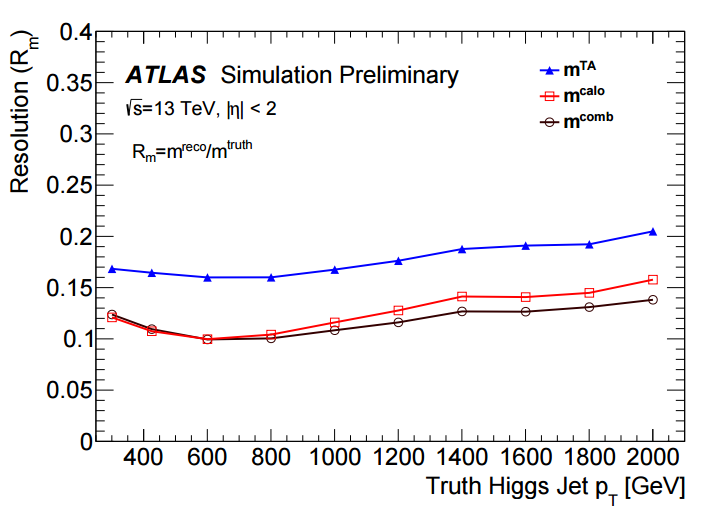
\includegraphics[width=0.7\textwidth]{jet_part/mta/higgsmta.png}
%   \caption[Performance of the $\mta$ with the boosted Higgs sample]{Performance of the $\mta$ with the boosted Higgs sample; the $\mta$ is the blue line, the $\mcomb$ will be described later in this chapter. From \cite{art39}. The FoM here is the resolution of the Response.}
%   \label{fig:mta4}
% \end{figure}



\subsection{The Track-Assisted Subjet Mass ($\mtas$)}\label{subsec:mtas_def}
In this section the main outcome of the optimization of the large-radius jet mas reconstruction is presented: the \textit{track-assisted subjet mass} ($\mtas$).
The main idea takes inspiration from the track-assisted mass: if one can use tracks to exploit the better angular resolution and correct the missing neutral component jet-by-jet, there is an additional information that can be used. The neutral fraction, in fact, varies stochastically not only per-jet basis, but even per-subjet basis, since each quark follows a different parton showering and hadronization process.
Correcting the missed neutral component per-subjet, should perform better already at an intuitive level, as it accesses information from jet substructure.
% There are few question in the definition of this mass observable, whose answers are in the next section:
% \begin{itemize}
%   \item Regarding the inputs:
%   \begin{itemize}
%      \item How to select the set of tracks to be used?
%      \item Which kind of subjet should be used?
%   \end{itemize}
%   \item Regarding the procedure
%   \begin{itemize}
  
%   \item How to associate the tracks to a subjet?
%   \item How to correct for the missed neutrals on a subjet basis?
%   \item How to add everything back together?
%  \end{itemize} 
 
% \end{itemize}

% Those details are given in the next subsection.


\subsubsection{Observable Definition: Inputs}
There are two inputs to the $\mtas$: tracks and subjets. The definition of the standard inputs are give here; alternative approaches are given in subsection \ref{sec:alternate}.

\paragraph{Tracks}
Only the tracks that satisfy the quality criteria and primary vertex association, described in the appendix \ref{sec:tracks}, are used.
The tracks are additionally required to be ghost associated to the subjets of the groomed jet; namely only the subjets which survived the trimming procedure and are described in the next subsection.
Ghost association provides a clear correspondence of tracks to the subjets set and was therefore chosen and preferred to other kind of assignments.

\paragraph{Subjets}

The choice of subjets follows a simple requirement: we want to take those which most likely come from the hard-scattering. This means that the choice of taking them after grooming is strongly favored.

As grooming technique used, the trimming was preferred as being the standard in ATLAS and the most flexible one for optimization studies.

The standard version of the trimming uses the k$_t$ reclustering algorithm with radius of 0.2, with the transverse momentum ratio $f_{cut}$ at 5\%.

As shown later, this is also the optimal configuration for subjets.

\subsubsection{Observable Definition: Procedure}
% As it will be shown and already stated in the introduction, the TAS procedure is being utilized with the Energy Correlation Functions and the n-Subjettiness. The four-momentum scheme which was described above and which was adopted as standard for the production of the $\mtas$ observable historically and also because of higher versatility and feasibility of implementation cannot be applied for those variable. The variable of interest to be modified which enters the computation of the ECF and n-Subjettiness is in fact the momentum.

% The procedure of assisting the tracks with the subjets or TAS is utilized both for the Energy Correlation Functions and the n-Subjettiness. However for these substructure variables the historically first procedure which was adopted, i.e. assisting the Track-Jets and rescaling the mass, is not possible because of simple cancellation in the observable definition. 

There are two ways of subjet assisting the tracks for the calculation of the $\mtas$: assisting track-jets changing the mass or assisting single tracks changing the transverse momentum. The first approach was the first one also historically, adopted because of higher versatility and feasibility of implementation. The second approach was also was found to be equivalent to the first (See \cite{presentation} and Figure \ref{fig:sascha}).

For the substructure variable, however, the first approach cannot be used because of simple cancellation in the computation of the variable.

To generalize the scheme adopted for both, tracks should be assisted singularly. In this note will be shown the $\mtas$ obtained assisting track-jets, since the differences are negligible as also shown in Figure \ref{fig:sascha}.

\begin{figure}[!ht]
  \centering
      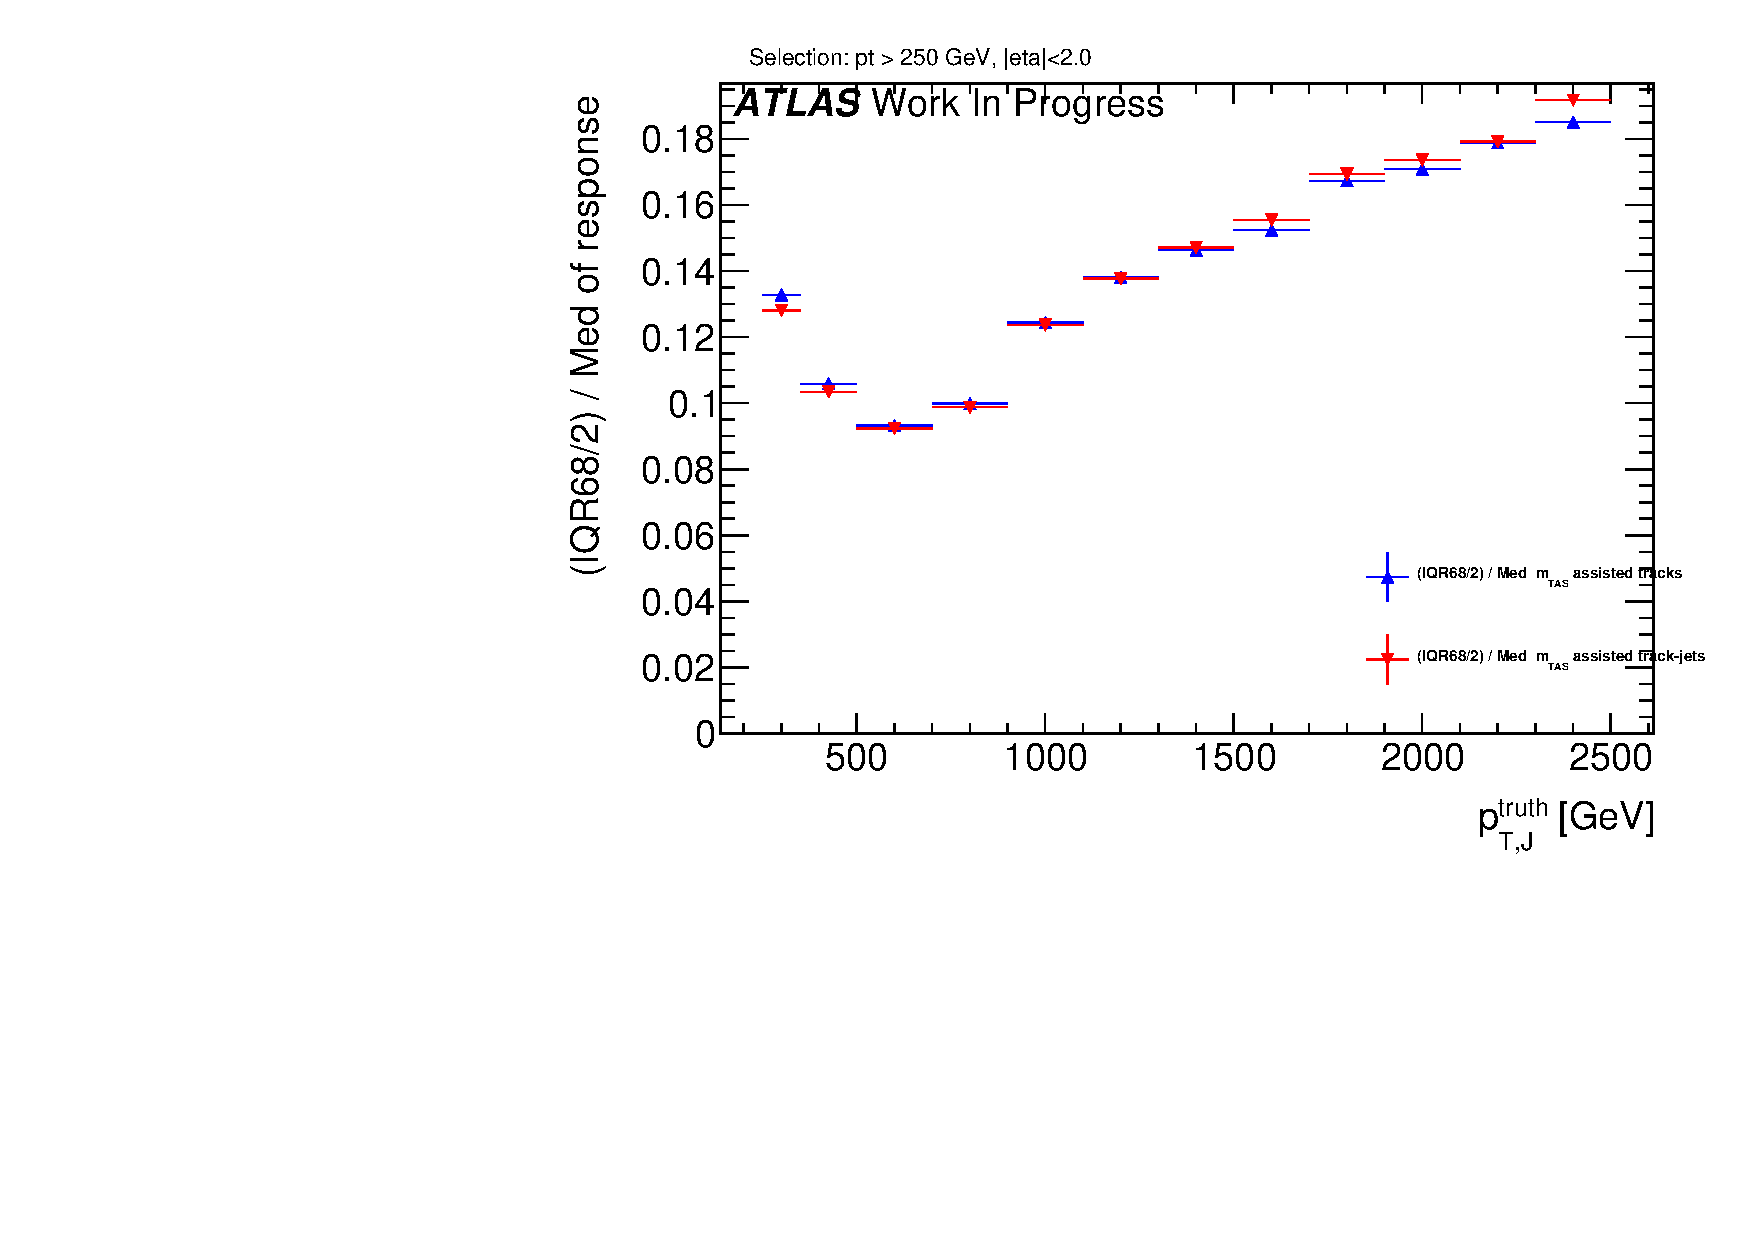
\includegraphics[width=0.55\textwidth]{jet_part/71graphcftr_h_JetRatio_mJ12CALOIQRoMwsecondApproach.pdf}
  \caption[Equivalence of approaches]{Performance of the $\mtas$ variable for the two approaches described in this section: assisting the track-jets in red and assisting single track in blue for $W/Z$ decays. They are performing almost identically throughout the entire spectrum of transverse momentum. For the computation of the track-assisted subjet variable presented in this document, the first method is being used, because of simplicity of implementation and higher versatility; for the computation of the subjet assisted substructure variables the second one is used. The y-axis is explained in the following section.}
  \label{fig:sascha}
\end{figure}


\paragraph{Assisting Track-Jets}
\label{sec:mtas}
Having tracks and subjets now well defined, we can describe the recipe to produce the $\mtas$. For brevity we will call the subjets SJ in the formulae below. 

As said, the tracks are the ones ghost-associated to the subjets; however, tracks which fall inside the area of the large-$R$ jet, but not inside the subjets area, are still much probably coming from the hard-scattering. They are then associated again to the closest subjets via $\Delta R$ association.

Each subjet will have at this point some tracks associated via ghost-association and some other via $\Delta R$ (which are maximally 5\%). We call this set of tracks, a ``custom'' Track-Jet or TJ.

\begin{figure}[!ht]
  \centering
      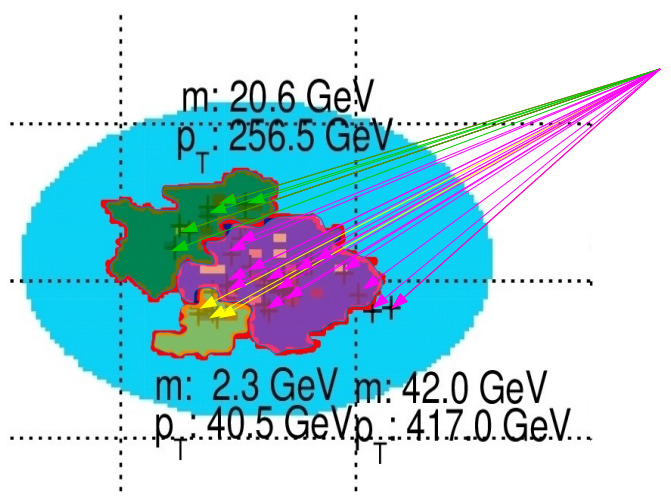
\includegraphics[width=0.6\textwidth]{jet_part/mtas/mtas.png}
  \caption[Pictorial event display]{Pictorial event display showing the $\eta$ $\phi$ region of a large-$R$ anti-k$_t$ trimmed jet, (in blue the catchment area of the anti-k$_t$) showing the different k$_t$ subjets: they are highlighted in green, fuchsia and yellow. The associated track-jets (here indicated as arrows pointing the calorimeter area) are colored with the same color of the correspondent subjet. Some tracks associated with $\Delta R$ procedure can be seen in the fuchsia subjet. The transverse momenta and mass values are also shown for the subjets.}
  \label{fig:mtas1}
\end{figure}

At this point, the one-to-one correspondence is preserved (for each SJ there is one and only one TJ), and we can move on correcting the neutral fraction.

Getting inspired from the formula $m^{TA}=p_T^{calo}/p_T^{track}\times m^{track}$, we would like to replicate this at subjet level, i.e.

$$\mtas="\sum_{SJ}"\frac{p_T^{SJ}}{p_T^{TJ}}\times m^{TJ}$$

Where the summation symbol between quotation mark symbolize that the sum must be intended at 4-vector level: since now we are working inside the subjets, in fact, we need to change the subjet's 4-vector itself and not only the mass. If we call $p_\mu^{TJ}$ the Lorentz vector of the track-jet, 

$$p_\mu^{TJ} = \spvec{m^{TJ};p_T^{TJ};\eta^{TJ};\phi^{TJ}} \to p_\mu^{TA}=\spvec{m^{TJ}\times\frac{p_T^{SJ}}{p_T^{TJ}} ;p_T^{SJ};\eta^{TJ};\phi^{TJ}} $$
 
where $p_\mu^{TA}$ is the track-assisted subjet's 4-vector. If we label $i$ the $i$-th track-jet of the $N$ ones present in the large-$R$ jet,

$$ \mtas=\sqrt{\left(\sum_i^N p^{TA} \right)_\mu \left(\sum_i^N p^{TA} \right)^{_\mu}} $$

\paragraph{Assisting Single Tracks}
\label{sec:tas}

This correction is now applied on single track rather than the whole track-jet and on the transverse momentum, not the mass.
The TAS correction reads:

$$p_\mu^{track} = \spvec{m^{track};p_T^{track};\eta^{track};\phi^{track}} \to p_\mu^{TA}=\spvec{m^{track} ;p_T^{track} \times\frac{p_T^{SJ}}{p_T^{TJ}};\eta^{track};\phi^{track}}$$

The correction factor $\frac{p_T^{SJ}}{p_T^{TJ}}$ refers to the $\pt$ of the subjet in which the track is associated and the $\pt$ of the track-jet associated to it.

% This momentum correction was studied with previous versions of the $\mtas$ and the difference with the stardard approach was found to be negligible \cite{presentation}.

As before, these four-momenta are then summed together to give this alternative definition:

$$ \mtas=\sqrt{\left(\sum_i^M p^{TA} \right)_\mu \left(\sum_i^M p^{TA} \right)^{_\mu}} $$

where now the sum refers from the first to the M-th tracks associated to the large-$R$ jet.


An important remark is that, in the case of a large-$R$ jet with only one subjet, the $\mtas$ has exactly the same definition of the $\mta$. This implies, since the angular separation of the decay product scales inversely with $\pt$, that the performance should approach the one of the $\mta$ at very high transverse momenta. However, the space for improvement is precisely in the low-intermediate $\pt$ regime.


\subsection{The Combined Mass}
\label{subsec:comb}


Since the calorimeter large-$R$ jet mass is not explicitly used in the track-assisted (subjet) mass, it may be possible to improve the performance creating a new observable which combines both mass definitions.
This is discussed in great details in the BOOST 2016 CONF Note \cite{art35}.


% \begin{figure}[!ht]
%   \centering
%       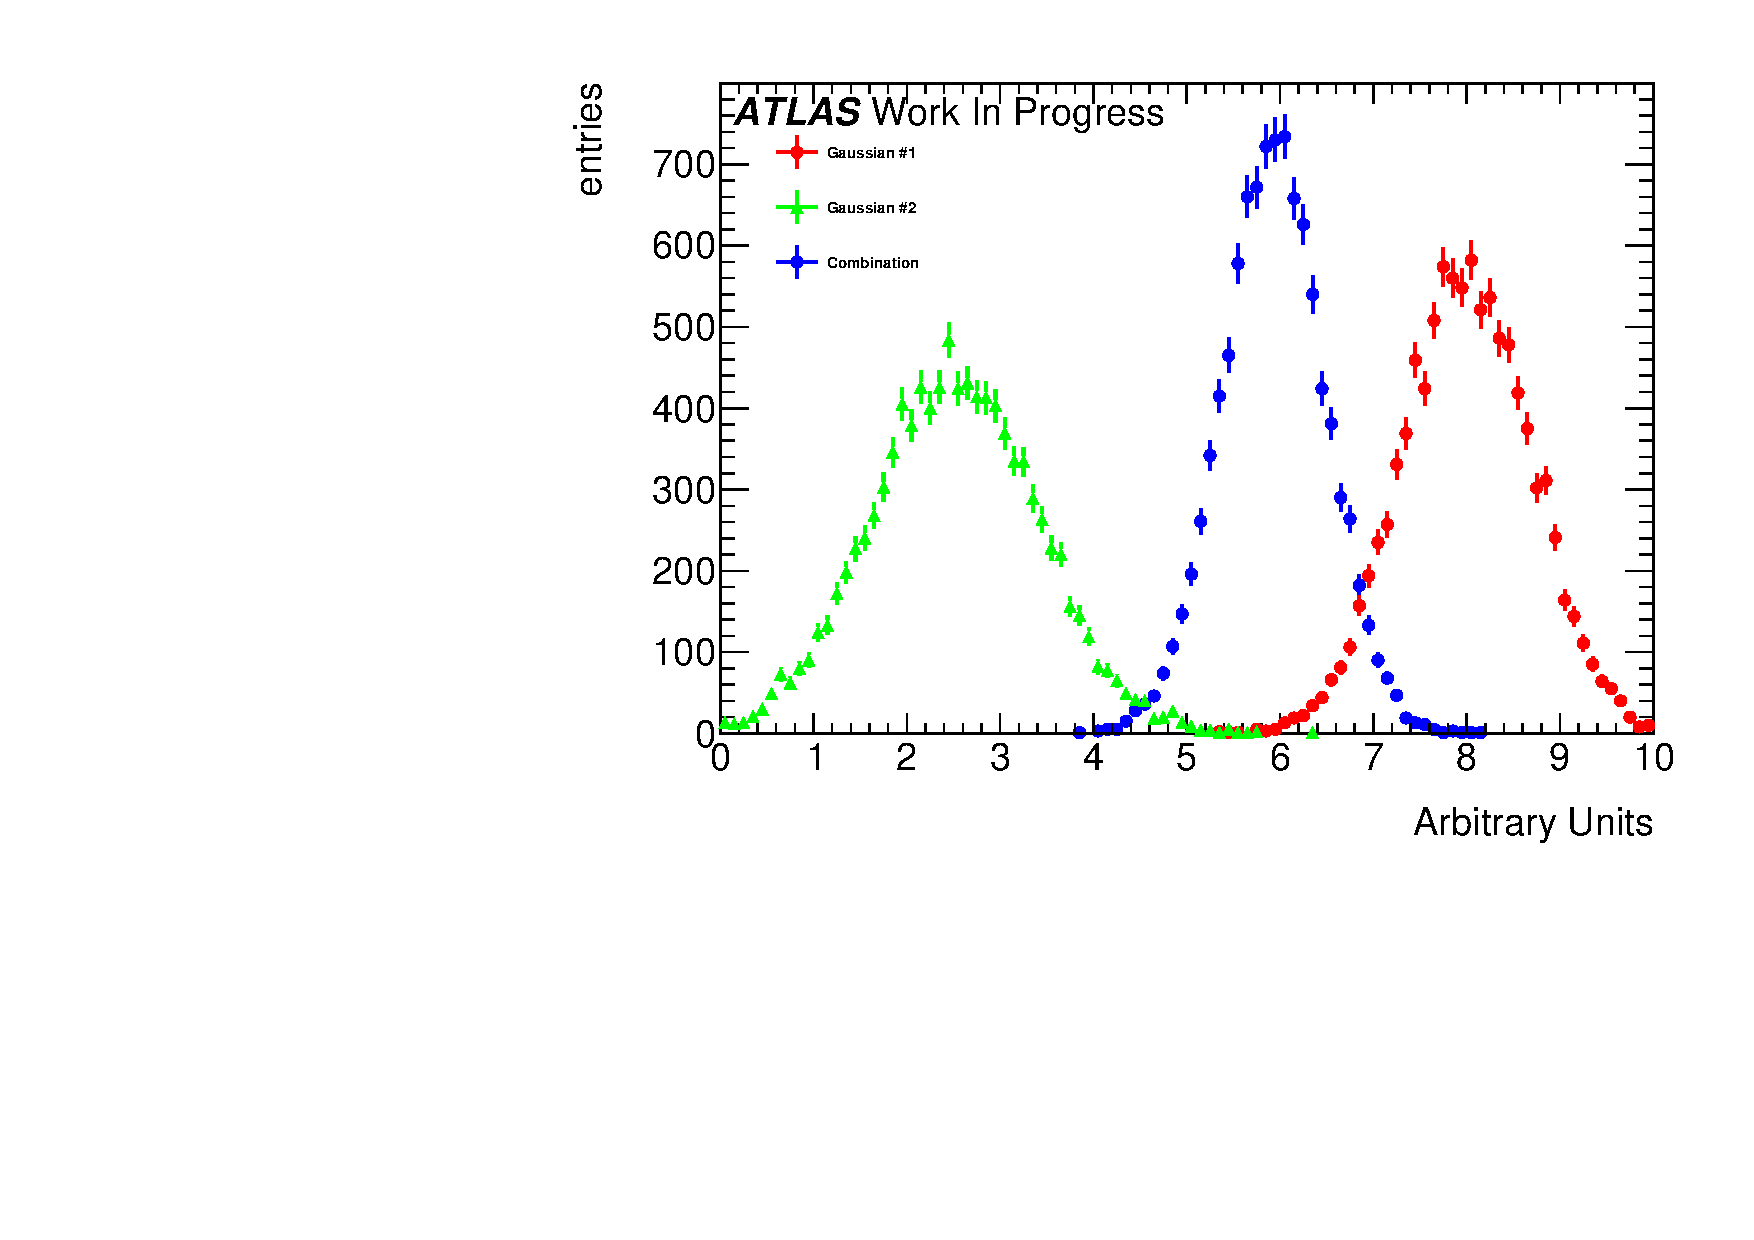
\includegraphics[width=0.7\textwidth]{jet_part/mcomb/example.pdf}
%   \caption[Toy example of Gaussian combination]{A toy example of the combination of two independent Gaussian observables, in red and green, and their combination, in blue. It can be seen that the combination has a smaller width.}
%   \label{fig:mcomb1}
% \end{figure}

% This is true for both the $\mta$ and the $\mtas$; their combination with $\mcal$ is introduced in the next subsections.
% Provided that the two observables are nearly independent (correlation coefficient are around 30\%, see Figure \ref{fig:mcomba1} in the Appendix), due to the approximate Gaussian nature of the $\pt$ and mass response, the optimal combination of the two is linear\footnote{If the joint distribution of the responses is Gaussian, then one can write their probability distribution function as $f(x,y)=h(x,y)\times \exp[A(\mu)+T(x,y)\mu]$, where $x$ is the calorimeter-based jet mass response, $y$ is the track-assisted jet mass response,
% $\mu$ is the common average response, and $h$, $A$,$T$ are real-valued functions. This form shows that the distribution is from the exponential family and therefore $T$ is a sufficient statistic. Since the natural parameter space is one-dimensional, $T$ is also complete. Therefore, the unique minimal variance unbiased estimator of $\mu$ is the unique unbiased function of $T(x, y) =x/\sigma^2_x \times + y/\sigma^2_y$.
% See e.g. Ref. \cite{statistic} and \cite{art35} for details.}.
% An example is provided in Figure \ref{fig:mcomb1}.


\subsubsection{Combination $\mta-\mcal$ }

For the $\mta-\mcal$ combination the observable are considered nearly independent, then
\begin{equation}\begin{split}
 \mcomb= a\times \mcal + b \times \mta,\\
 a=\frac{\sigma_{calo}^{-2}}{\sigma_{calo}^{-2}+\sigma_{TA}^{-2}} \qquad b=\frac{\sigma_{TA}^{-2}}{\sigma_{calo}^{-2}+\sigma_{TA}^{-2}}
\end{split}
\label{eq:mtacomb}
\end{equation}
where $\sigma_{calo}$ and $\sigma_{TA}$ are the $\mcal$'s and $\mta$'s resolution functions. The $\mcomb$ then is the $\mta-\mcal$ combination.
The weights are here and also afterwards computed from the mass response distribution; the sigma parameter corresponds to the width of the Gaussian distribution, which is estimated using the InterQuantile range. 

\subsubsection{Combination $\mtas-\mcal$ }

There is a main difference between the $\mtas$ and $\mta$ when it comes to combination: since the $\mtas$ is using subjet level information but $\mta$ not, the correlation with the $\mcal$ is expected to be higher.
This can be seen e.g. in the plots in Figure \ref{fig:mcomb2} (additional plots shown in Figure \ref{fig:mcomba2} in Appendix), where the correlation is not only higher for the simple $W/Z$ and Higgs jets, but above 50\% for tops. The assumption of independent variables here falls, since the observable are only approximately Gaussian. The Ansatz is to take into account the correlation via the formula:
\begin{equation}
\begin{gathered}
\mcombtas= w\times\mcal + (1-w)\times\mtas,\\
w=\frac{\sigma_{TAS}^2-\rho\sigma_{calo}\sigma_{TAS}}{\sigma_{calo}^2+\sigma_{TAS}^2-2\rho\sigma_{calo}\sigma_{TAS}}
\end{gathered}
\label{eq:mtascomb}
\end{equation}
% 
where now $\mcombtas$ is the new $\mtas-\mta$ combination. This expression reduces then to the form:
\begin{equation}
\begin{gathered}
\mcombtas= a\times\mcal + b\times\mtas,\\
a=\frac{\sigma_{TAS}^2-\rho\sigma_{calo}\sigma_{TAS}}{\sigma_{calo}^2+\sigma_{TAS}^2-2\rho\sigma_{TAS}\sigma_{calo}}\qquad b=\frac{\sigma_{calo}^2-\rho\sigma_{calo}\sigma_{TAS}}{\sigma_{calo}^2+\sigma_{TAS}^2-2\rho\sigma_{TAS}\sigma_{calo}}
\end{gathered}
\end{equation}
which reduces to equation \eqref{eq:mtacomb} after simple algebra for the case when $\rho=0$. Of course, this value can be set to the value of the specific sample considered, or to an average of 0.3 if one wants to give a definition generally valid for all the cases considered; in this case, the performance would be slightly sub-optimal.

\paragraph{Procedure}
The procedure of producing the $\mcombtas$ is defined as follows:
\begin{enumerate}
 \item For the given sample, the $\mtas$ and $\mcal$ are calculated;
 \item The mass responses are also produced for the given ranges of $\pt$;
 \item For each of these responses, the value of the $\frac{68\% \: \textrm{IQnR}}{2}$ (described in the next subsection and identified as the $\sigma$ in Eq \ref{eq:mtascomb}) is calculated and stored;
 \item The average correlation factor of 0.3 (an average value for the samples considered) is assumed;
 \item With the formula \ref{eq:mtascomb}, $\mcombtas$ is calculated using the $\mtas$, $\mcal$ and the values stored in step 3.
\end{enumerate}

% A remark on the procedure: the step 3. uses values of the IQnR because this was showed to be a more robust way to look at the response and fit-independent. The $ \frac{68\% \:\textrm{IQnR}}{2}$
% For step 4. the correlation factor was decided to be an average of the samples considered.

In this note, the IQnR weights are produced for each sample specifically. In order to give a sample-independent definition of the $\mcombtas$, following also the procedure adopted for the $\mcomb$, these weights could be taken from a QCD multijet sample and applied indiscriminately to the particular case. Here of course the performance would be again sub-optimal, being the variable not developed in an ad-hoc way for each signal sample, but from QCD multijet only.

Throughout the results presented in the following sections, both observables were calculated with ad-hoc weights. Quantitative statements between them would still hold in the case of QCD weights. However, when confronting e.g. $\mtas$ with them it has to be kept in mind that in this case their performance is overestimated, since this choice, although being more general, would perform slightly worse.

\begin{figure}[!ht]
  \centering
      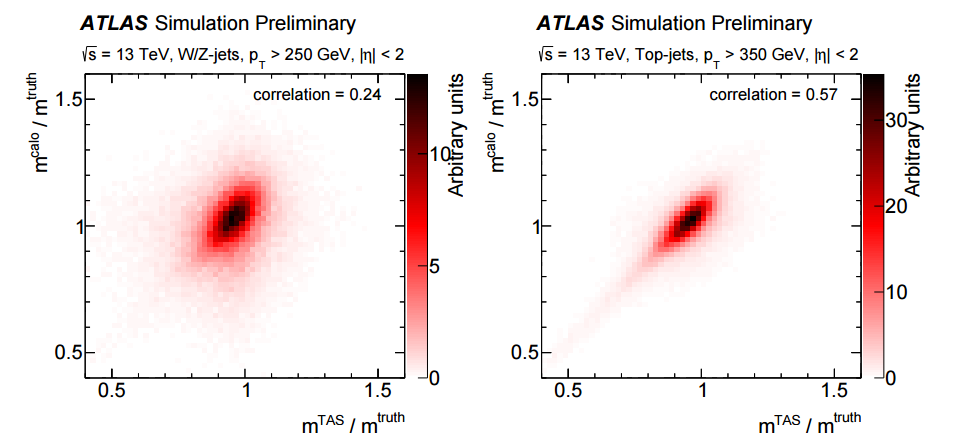
\includegraphics[width=0.7\textwidth]{jet_part/mcomb/mcomb2.png}
  \caption[$\mcal$ and $\mtas$ correlation plots]{The calorimeter based jet mass mass response versus the track-assisted subjet mass response, on the left for $W/Z$ decays and on the right for tops decays.}
  \label{fig:mcomb2}
\end{figure}



